\section{Calculs de statique et de dynamique}
\label{meca}
Le but est de déterminer une vitesse max en virage sans renversement du chariot; et une vitesse max en ligne droite garantissant une décélération sans glissement du colis.

Pour cela, nous utiliserons des équations de dynamique, ce qui suppose de modéliser le chariot. Nous ferons donc des hypothèses sur sa forme géométrique et la répartition de sa masse. Ensuite, nous avons obtiendrons par des théorèmes les équations attendues: vitesse max en ligne droite, vitesse max en virage. Enfin, nous vérifierons l'adéquation de ces résultats avec des mesures sur un modèle physique de chariot que nous avons construit (nous l'appelerons le prototype).

\label{hypProtoCommeChariot}
Mais la validation des hypothèses sur le chariot élévateur par des mesures sur notre prototype mécanique nécessite de supposer que notre prototype mécanique est lui-même un bon modèle qui se comporte comme un chariot élévateur. Elle permet en fait de généraliser l'ensemble des productions de notre TX (modèles mécaniques et numériques, voir \ref{proto}) à tous les chariots élévateurs, et à tous les véhicules verticaux, fins et avec un centre de masse haut. Elle pourrait être appuyée par des arguments théoriques, mais le seul argument que nous fournirons est le fait que toutes les dimensions sont du même ordre de grandeur. Cette hypothèse est très forte, mais elle n'est pas critique: si elle n'était pas vraie, cela signifierait que nos productions ne seraient valables que pour notre prototype.

\subsection{Description de l'étude}
\begin{itemize}
	\item Le hangar est muni du repère $R_g = (O,\vec x_g, \vec y_g, \vec z_g)$.
	\item Le chariot $(0)$ est animé d'un mouvement de rotation par rapport au sol dont le centre instantané de rotation est $O$.
	\item Le rayon de courbure de la trajectoire du point C dans $R_g$ est $R$.
	\item Le repère lié à $(0)$ est $R_0 = (O, \vec x_0, \vec y_0, \vec z_0)$ tel que $\vec z_0 = \vec z_g$ et on note $\theta = (\vec x_g, \vec x_0) = (\vec y_g, \vec y_0)$.
	\item Donc $\vec{OC} = R \cdot \vec x_0$. On remarque bien que $R_0$ est mobile par rapport à $R_g$.
	\item On considère que les frottements du colis $(1)$ l'encastrent avec le chariot $(0)$.
	\item Le repère lié au colis est $R_1 = (C, \vec x_1, \vec y_1, \vec z_1)$ et tant qu'il n'y a pas glissement du colis, $\vec e_1 = \vec e_0 \forall e \in \{x,y,z\}$.
	\item Le centre de gravité du colis est $G$ tel que $\vec{CG} = e\cdot\vec z_1$. La masse du colis est m.
	\item Le contact entre le colis et le chariot est modélisé par une liaison plan à plan, avec un coefficient de frottement $\mu$.
\end{itemize}
\begin{figure}
	\centering
	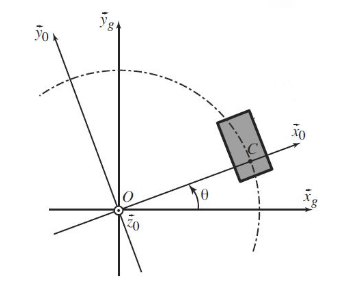
\includegraphics[height=5cm]{schema_chariot3}
	\caption{Le virage du chariot paramétré}
	\label{fig:schemaChariot3}
\end{figure}
\subsection{Calculs}
\paragraph{Vitesse de $G$ dans $R_g$}
\[\vec{OG} = \vec{OC} + \vec{CG} = R_c \cdot \vec x_0 + e\cdot \vec z_1 = R_c \cdot \vec x_0\]
\[\vec v(G/R_g) = \frac{d\vec{CG}}{d_t}_{R_g} = \dot \theta \vec z_0 \wedge R_c \dot \theta \vec y_0 = -R_c \dot \theta^2 \vec x_0 \]
Avec $ V = R_c \dot \theta$ on obtient:
\begin{equation}
	\vec v(G / R_g) =V \vec y_0
\end{equation}
